\documentclass[11pt, a4paper]{article}

\usepackage{times}
\usepackage[left=1.6cm, top=1.5cm, text={18cm, 24.7cm}]{geometry}
\usepackage{graphics}
\usepackage{pict2e}

\title{Implementační dokumentace k 2. úloze do IPP 2022/2023}
\author{Jméno a příjmení: Denys Petrovskyi\\ Login: xpetro27}
\date{}

\begin{document}

\maketitle
\section{Program structure}
At the beginning of the code global variables and 2 classes(\verb|Instruction| and \verb|Argument|) are initialized. First
one is used to store all the data about instructions that program will get, second class is used to store data about 
arguments that each instruction has. After classes there are functions, all the analysis is in function called 
\verb|interpret()|, other functions are helping it.
\section{Implementation procedure} 
\subsection{Main function}
Program starts in \verb|main| with parsing arguments. To implement this was used import \verb|sys|. After that program starts working 
with source file. Using import \verb|xml.etree.ElementTree| and loops program goes through \emph{XML} code and detects errors,
then all the instructions and arguments are being written to objects of classes, objects of class \verb|Instruction|
are being added to the \verb|listOfInstructions|.
\subsection{Preperation before analysis}
After that function \verb|mySort()| is being called. Its purpose is to sort all the instructions based on their order
which was given in \emph{XML} code, so they would have the right order in the list.
Then there is function called \verb|fisrt_walktrough()|, it is being called before the main analysis starts,
so it can detect all the initialized labels and add the to the list.
\subsection{Interpret}
If the previous code passes without errors, the function \verb|interpret()| starts. Using a \emph{for} loop 
it goes through every instruction in the \verb|listOfInstructions| and then depending on the name of each instruction it 
performs analysis. There are several functions that help with analysis:
\begin{itemize}
    \item \verb|check_arg_amount()| checks if the right amount of arguments instruction has.
    \item \verb|check_var_existance()| function goes through each frame (\emph{global, local, temporary}), which are defined as dictionaries,
    and looks for a specified variable.
    \item \verb|check_var_value()| checks if variable has a value and returns it if such exists. Works similarly as \verb|check_var_existance()|.
    \item \verb|check_var_type()| gets type of variable and returns it.
    \item \verb|control_escapeseq()| is created to change all the escape sequances in string to \emph{ASCII} symbol.
    \item \verb|find_inst_by_order()| function gets the instructions position in \verb|listOfInstructions| based on its order.
    \item \verb|add_value_to_var()| adds value to the variable.
\end{itemize}
After processing all the instructions, program ends.
\newpage
\begin{figure}[ht] 
    \begin{center}
        \scalebox{0.4}{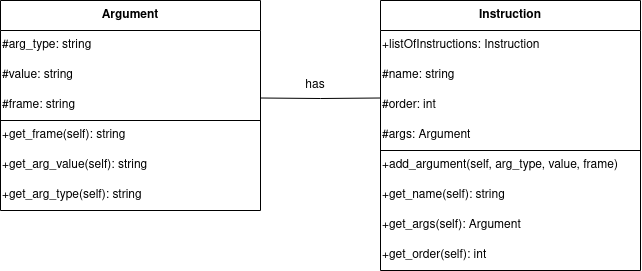
\includegraphics{uml.png}} 
        \caption{UML class diagram}
    \end{center}
\end{figure}

\end{document}